\documentclass{article}
\usepackage{amsfonts}
\usepackage{amsthm}
\usepackage{amssymb}
\usepackage{amsmath}
\usepackage{graphicx}
\usepackage{subcaption}
\usepackage{xcolor}

\newcommand{\new}[1]{
    \vspace{2mm}
    \noindent
    \textbf{
    \underline{#1}}
}

\def\calO{{\mathcal{O}}}
\def\th{{\theta}}
\def\_{{\hspace{1mm}}}
\def\<{{\langle}}
\def\>{{\rangle}}


\newcounter{problemcnt}
\setcounter{problemcnt}{0}

\newcommand{\Problem}{{
    \vspace{5mm}
    \stepcounter{problemcnt}
    \noindent
    \arabic{problemcnt}. 
}
}

\newcommand{\nProblem}[1]{
    \vspace{5mm}
    \noindent
    \setcounter{problemcnt}{#1}
    \arabic{problemcnt}. 
}


\newcommand{\Proof}{{
    \vspace{2mm}
    \noindent
    \textbf{
    \underline{Proof}}
}
}

\newcommand{\textOr}{
    {
        \hspace{5mm}
        \textrm{or}
        \hspace{5mm}
    }
}

\newcommand{\textAnd}{
    {
        \hspace{5mm}
        \textrm{and}
        \hspace{5mm}
    }
}

\def\twobytwoMat(#1, #2, #3, #4){
    {
        \begin{bmatrix}
            {#1} & {#2}\\
            {#3} & {#4}
        \end{bmatrix}
    }
}

\def\twobyoneMat(#1, #2){
    {
        \begin{bmatrix}
            {#1}\\
            {#2}
        \end{bmatrix}
    }
}

\def\twobytwoDet(#1, #2, #3, #4){
    {
        \begin{vmatrix}
            {#1} & {#2}\\
            {#3} & {#4}
        \end{vmatrix}
    }
}



\begin{document}
\begin{center}
\LARGE
PHYS 202 HW4

\Large
Daniel Son
\end{center}

\normalsize 


\new{Q1} 
Two masses $m_1, m_2$ are connected by a spring with a spring constant 
$k$. 

a) Write out a general solution for the position of the two masses. 

b) Find a specific solution for $x_1(0) = x_2(0) = 0$ and $v_1(0) = v$

c) Sketch $x_1(t)$ and $x_2(t)$. 


\new{Solution}

Each of the masses must have a linear term which 
describes the constant velocity of the center of mass. 
Also, each mass must have a oscillating term. By Newton's 2nd law, 
we write 

\[
    \ddot{x_1} = - k(x_1 - x_2) \textAnd 
    \ddot{x_2} = - k(x_2 - x_1)
\]

Also, in light of our previous observation, we guess the solution 
to be in the form of 
\[
    x_1 = Re[Ae^{i\omega t} + Ct]
    x_2 = Re[Be^{i \omega t} + Ct]
\]
It is possible to include a constant term, but it is possible to 
redefine $x_1, x_2$ to be zero at the defined place of axis, so 
we discard the extra variables for simplicity. 

Complexify the equation and plug them into the coupled differential 
eqation. 
We obtain the following matrix equation. 

\[
    k\twobytwoMat(-1/m_1, 1/m_1, 1/m_2, -1/m_2) \twobyoneMat(A, B) 
    = -\omega ^2 \twobyoneMat(A, B)
    \textOr 
    k\twobytwoMat(1/m_1, -1/m_1, -1/m_2, 1/m_2) \twobyoneMat(A, B) 
    = \omega ^2 \twobyoneMat(A, B)
\]



The eigensystem of the 2x2 matrix narrows down the candidates 
of the angular frequency and the amplitude $A, B$. According 
to mathematica, the eigensystem is as follows. 

\begin{center}
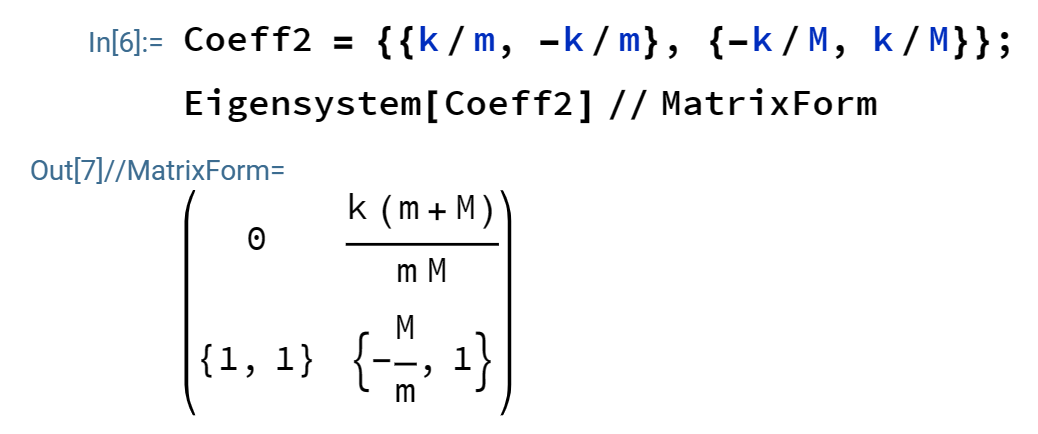
\includegraphics[width = .5\linewidth]{Fig1.png}
\end{center}

Thus, we obtain the two possible solutions. 
\[
    (\omega, A, B) = (0, G, G) \textOr (\sqrt{\frac{k(m+M)}{mM}}, -MG/m, G)
\]
Where $G$ is an arbitrary constant. The two restrictions 
does not provide constraints on $C$. 
Also, we defined the initial position to be zero at $t = 0$. 
Thus, we compute the imaginary part of the complexified equation 
instead of the real part. 
We write the general solution 
as follows. 

\[
    \boxed{
    (x_1, x_2) = (Ct, Ct) 
    \textOr 
    (-\frac{MG}{m}\sin(\sqrt{\frac{k(m+M)}{mM}} t)+ Ct, G\sin(\sqrt{\frac{k(m+M)}{mM}} t)+ Ct)
    }
\]


We simplify the equation by using the definition of reduced mass. 
\[
    \mu := \frac{mM}{m + M}
\]

\[
    \boxed{
    (x_1, x_2) = (Ct, Ct) 
    \textOr 
    (-\frac{MG}{m}\sin(\sqrt{k/ \mu} t)+ Ct, G\sin(\sqrt{k/\mu} t)+ Ct)}
\]

To compute the particular solution, compute the time derivative 
of $x1$ and apply the condition $\dot{x_1}(0) = v$. 

\[
    \dot{x_1}(0) = -\frac{MG}{m} \sqrt{\frac{
        k(m + M)
    }{mM}} = v
\]


With some algebra, 
\[
    G = -v\sqrt{\frac{m^3}{kM(m+M)}}
    \]


Thus 
\[
    G = -v
\]





\end{document}